For each patient we hereby present a performance result both for
classification and regression.

For classification, the performance index is the \emph{weighted}
percentage of correctly guessed labels, that is, the average of the
percentages for each label $i$, divided by the number of labels $i$ in
the testing set. This measure, as opposed to the more standard ratio
of correctly guessed labels, has the advantage of adjusting the
importance of each label according to how often it appears in the
testing set. For example, in general there are more $0$ labels in any
testing set than other labels, since $0$ appears both at the beginning
of the experiment and in-between the grasps, as it represents
rest. Therefore this label must be weighted \emph{less} than the
others, since it is more easily found in the testing set.

For regression, the performance index is the standard Pearson
correlation coefficient evaluated between the predicted force signal
and the real one (remember that we work in real-time, so that this
measure of correlation really is a measure of temporal
correlation). The choice of the correlation coefficient, as opposed to
the more standard mean-square error, is suggested by a practical
consideration: when driving a prosthesis, or even a non-prosthetic
mechanical hand, we are not interested in the absolute force values
desired by the user/subject, since mechanical hands usually cannot
apply as much force as human hands do, for obvious safety
reasons\footnote{or, e.g., in teleoperation scenarios, they could be
able to apply \emph{much more} force than a human hand can.}. We are
rather concerned about getting a signal which is \emph{strongly
correlated} with the patient's will.

As is standard in machine learning, each data set was split in $5$
folds and cross-validation was performed on it; this makes the
evaluation robust against the problem of over-fitting. We employed a
well-known freely available SVM package, \emph{libsvm} v2.83
\cite{ChangL01}, in the Matlab wrapped flavour, with a Gaussian
kernel. This particular kind of SVM, in our case employing the
so-called Gaussian or Radial Basis Function kernel, requires setting
two \emph{hyperparameters}, called $\gamma$ and $C$, which were found
by grid search using the aforementioned performance indexes.

Table \ref{tab:results} shows the main results obtained by the SVMs.

\begin{table}[!ht] \centering
  \caption{Classification/regression performance for each subject
    (row) and modality (column).}
  \begin{tabular}{|c|r|r|r|}
    \hline
                & Imitation & Bilateral & Mirror \\
    \hline
    Subject $1$ & $93.11\%$ / $0.96$ & $90.41\%$ / $0.95$ & $82.39\%$ / $0.93$ \\
    Subject $2$ & $88.67\%$ / $0.86$ & $95.98\%$ / $0.96$ & $96.07\%$ / $0.94$ \\
    Subject $3$ & $84.07\%$ / $0.81$ & $92.40\%$ / $0.92$ & $91.98\%$ / $0.91$ \\
    \hline
  \end{tabular}
  \label{tab:results}
\end{table}

The first consideration is that for each subject, at least one
modality produces excellent results, both in classification and
regression. Subject $1$ works best by imitation, whereas subjects $2$
and $3$ exhibit best results via bilateral action and mirror-box. If
we consider the modality with the best results for each subject, we
get an average classification accuracy of $93.86\%$ and an average
regression correlation of $0.95$. The system can predict almost
perfectly, as is apparent from Figure \ref{fig:examples} in which a
comparison is shown between bits of real target labels and values and
the corresponding guessed targets.

It is unclear why modalities produce better or worse results according
to the subjects, but see Section \ref{sec:disc} for a couple of hints
on why this phenomenon appears.

\begin{figure*}[!ht] \centering
  \begin{tabular}{ccc}
    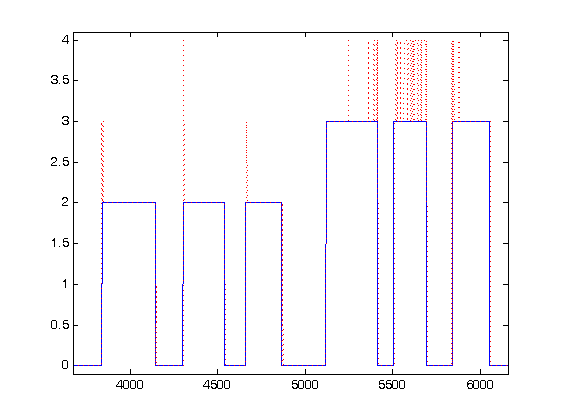
\includegraphics[width=0.3\textwidth]{figs/example1} &
    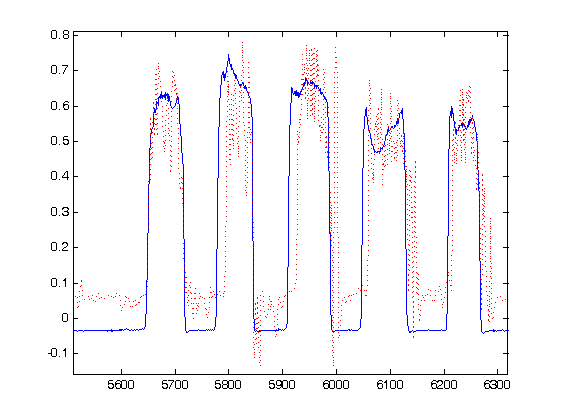
\includegraphics[width=0.3\textwidth]{figs/example2} &
    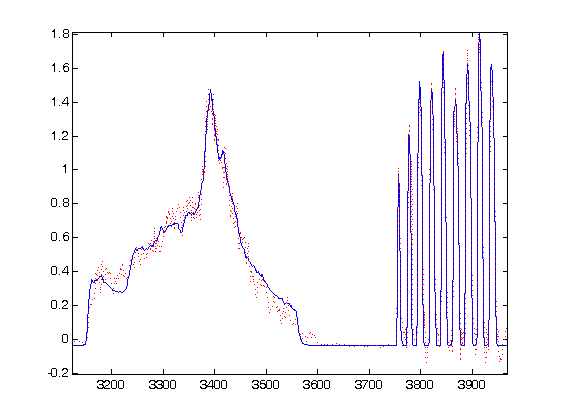
\includegraphics[width=0.3\textwidth]{figs/example3} \\
    $(a)$ & $(b)$ & $(c)$ \\
  \end{tabular}
  \caption{comparing true and guessed labels $(a)$ and force values
    $(b)$ and $(c)$. Notice, in panel $(a)$, that labels
    $3$ (pinch grip) are easily mistaken for labels $4$ (tripodal
    grip) but not to the point of hindering the performance of the
    system. Notice also, especially in panel $(c)$, the almost perfect
    correlation between force and guessed force, both during a slow
    buildup/release and during quick applications of force.}
  \label{fig:examples}
\end{figure*}

Consider the Figure, panel $(a)$: the major problem seems that of
pinch grips which get mistaken for tripodal grips, and this is
intuitively clear, since these two types of grips are quite similar
from an anatomical point of view. This fact is corroborated by the
fact that (consider Figure \ref{fig:PCA} again, pink and black dots)
the two grips lie, almost consistently, in the same regions of the
$2$-dimensional PCA-transformed input space.

\begin{figure*}[!ht] \centering
  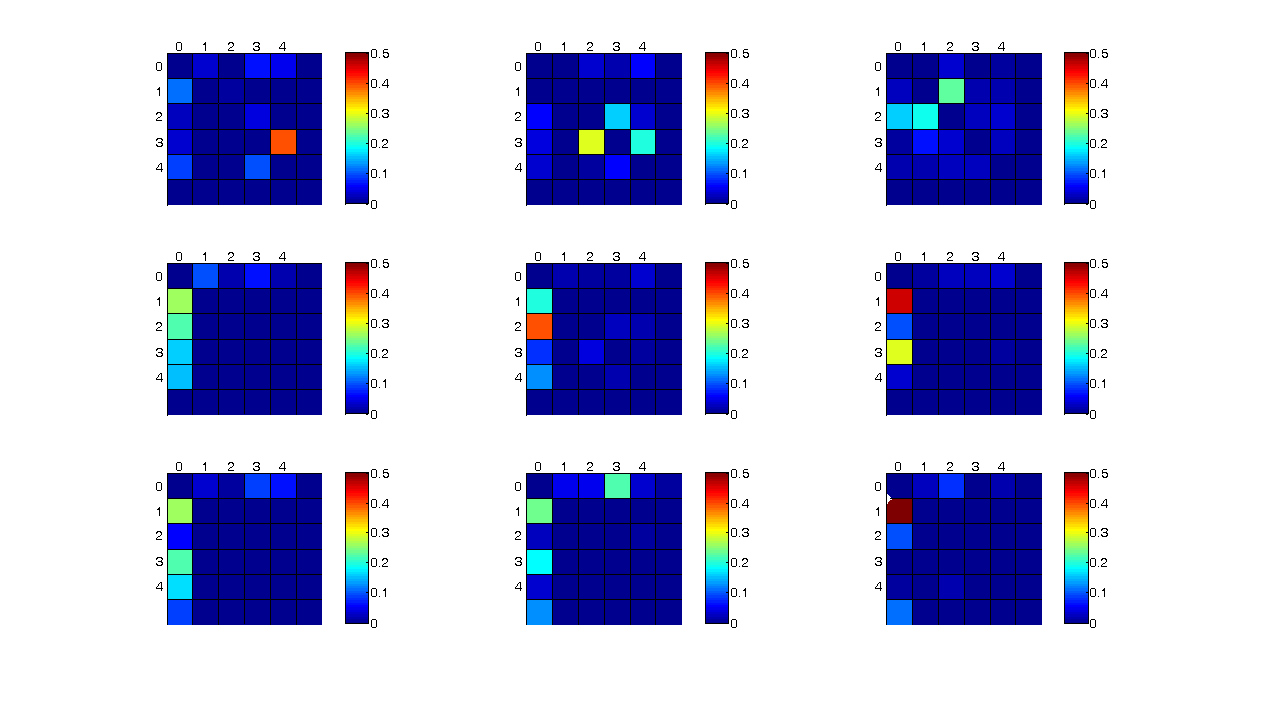
\includegraphics[width=\textwidth]{figs/confusion}
  \caption{confusion matrices for each subject / modality
    pair. Subjects are on each row, modalities are on each column. In
    each matrix $C$, the entry $C_{ij}$ denotes the fraction of labels
    $i$ which have been mistaken for $j$ over the total mistaken
    labels of that particular subject / modality pair. The diagonals
  of the matrices are, therefore, identically zero.}
  \label{fig:confusion}
\end{figure*}

Actually, the confusion matrices related with each subject / modality
pair (see Figure \ref{fig:confusion}) confirm this feeling only for
subject $1$ and only partially. Really, most mistakes in
classification involve label $0$, both in the sense that $0$ is
mistaken for something else and vice-versa (consider the first row and
first column of each matrix). This happens especially (consider rows
$2$ and $3$ of the Figure) for subjects $2$ and $3$, whereas subject
$1$ presents more uncertainty as far as other confusion pairs are
concerned. This phenomenon is also clearly justifiable, since
misclassifications involving label $0$ (the ``rest'' position) happen
at the onsets / endings of grips --- this is confirmed by visual
inspection, in the cases of modalities $2$ and $3$ (in modality $1$
the teacher was pressing the force sensor, so the data are unreliable
for this kind of analysis), and for subjects $2$ and $3$. In these
cases, willing to obtain an even more accurate classification rate,
one can think of using the regression system to guess when the
required force is above a reasonable threshold, and start the
classification only at that point, when the chance of mistaking the
posture / grip is close to zero. Also, in a practical setting, a
simple buffering strategy (i.e., considering a few samples before
switching category) would probably suffice to eliminate this problem
completely.

As far as regression is concerned, consider now Figure
\ref{fig:examples}, panels $(b)$ and $(c)$. If we neglect a
high-frequency oscillation, the guessed force values are essentially
replicating the true values --- again, there are different offsets,
but this is a direct result of choosing \emph{maximum correlation} as
the performance index. The signals in the Figure could easily be used
in practice after a simple linear transformation; the oscillation can
be removed by low-pass filtering the signal before sending it to the
control system of the prosthesis, or by relying on the
electro-mechanical time constants of the prosthesis itself, which
would probably be hardly capable of accurately following such a
high-frequency spurious signal. Notice in particular (panel $(c)$) how
the system is smoothly able to correctly guess both low-frequency
(left-hand side) and relatively high-frequency (right-hand side)
oscillations of the target value.

Inspection of the hyperparameters $C$ and $\gamma$ is useful to narrow
down the grid search and also to gather more abstract considerations
about the problems at hand. Here we have that, in classification, (the
logarithm of) $C$ is $2.17 \pm 0.83$ and $\gamma$ is uniformly
$2$. These numbers reveal that the problem is rather easy, since $C$
is set at a quite high value, and as well $\gamma$ is at the highest
possible value in our grid search range. As far as regression is
concerned, we find a similar pattern, with (the logarithm of) $C$
being $0.56 \pm 0.53$ and $\gamma$ being set, again, at $2$
uniformly. Regression as well seems an easy task for SVMs, which in
the end confirms the visual appearance of the PCA scatterplots of
Figure \ref{fig:PCA}.

One last hint at this comes from the analysis of the models
themselves. SVMs enjoy the property of building \emph{sparse}
solutions to the problems on which they are trained; this means that
the prediction function, for the selected kernel, both for
classification and regression, is a weigthed sum of Gaussian
functions. The Gaussians involved in the sum are centered around some
of the training samples --- the so-called \emph{Support Vectors}
(SVs), and their number is usually much smaller than the total number
of samples used in the training phase.

The sparsity of SVM models is extremely useful in our context, since
smaller models mean higher chance of miniaturising them and using them
in pratice. At the same time (see, e.g., \cite{v-edbed-82}), it is
well-known that the total number of SVs is inversely correlated to the
model's generalisation power, and therefore to its overall
performance. In our case, the percentage of SVs with respect to the
size of the related training sets is systematically low and strongly
inversely correlated with the perfomance attained. For classification,
the percentage is $20.55\% \pm 6.07\%$ with correlation to the
performance $-0.96$; for regression, we have $17.11\% \pm 9.53\%$ with
correlation $-0.93$.

In practical terms, let us consider, for example, the models obtained
for Subject $3$ via bilateral action, a case in which the performance
is excellent: the classification model has $2059$ SVs and the
regression model has $1324$, for a total memory occupancy (in Matlab)
of, in turn, $207$KB and $91$KB, which is small enough to fit on any
miniaturised device avaialble nowadays (see the next Section for more
details). Of course, things are supposed to get even \emph{better}
from this point of view, if we allow for a slightly worse performance
and employ a sparsification technique such as, e.g., uniformisation
\cite{2008.ICRA,2008.BioCyb}; such a technique is anyway needed when
we switch to a real online framework.
